\scanpage{31}

Supposons $j$ et $j'$ ainsi \unsure{choisis}. Si $j,j'$ sont injectifs, on en déduit une biextension \inserted{\figure{
\begin{tikzpicture}[baseline=(t.base)]\node (t) {canonique};\draw (0,0) ellipse (.8 and .22);\end{tikzpicture}}} de $(A,A')$, où $A=G/M$, $A'=G'/M'$. Dans le cas général, posons

\deleted{pour dire qu'on a une biextension de}
\[
A=\left[\underset{\text{deg.}\,-1}{M}\longrightarrow\underset{\text{deg}\,0}{G}\right]\ ;\qquad
A'=\left[M'\mathbin{-}G'\right].
\]

d'où
\diagram{\begin{tikzcd}[ampersand replacement=\&, row sep=small,column sep=small]
 \& \& A \arrow[dl,"1"'] \& \& \& \& A' \arrow[dl,"1"'] \& \\
\phantom{0} \& M \arrow[l,no head] \arrow[r] \& G \arrow[u] \arrow[r,no head] \& \phantom{0} \& \text{\unsure{cônes de morphismes}} \& M' \arrow[l,no head] \& G' \arrow[u] \arrow[l,no head] \&
\end{tikzcd}}

on va définir une \deleted{\unsure{biextension}} classe canonique
\[
\xi\in\operatorname{Ext}^1(A\mathbin{\overset{L}{\otimes}}A',G_m),
\]
jouant le rôle d'une biextension de $(A,A')$ par $G_m$.

Soit en effet \figure{\begin{tikzpicture}[baseline]\draw(0,.08)--(.1,.04);\draw(.16,.04)--(.26,.04);\draw(.31,.03)--(.43,.06);\draw(.53,.04)--(.82,.07);\draw(.94,.04)--(1.06,.08);\end{tikzpicture}}
\margin{\unsure{pourquoi ?}}
\figure{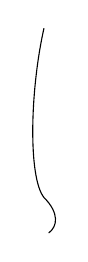
\begin{tikzpicture}\draw (0,2.4) .. controls (-.18,1.6) and (-.2,.5) .. (0,.25) .. controls (.2,.05) and (.17,-.12) .. (.06,-.2);\end{tikzpicture}}

\unsure{Soit}
\[
{}_nA\overset{\text{déf}}{=}\deleted{\unsure{R}}\underline{\operatorname{Ext}}^0(\unsure{\mathbb Z|\mathbf Z}/n\unsure{\mathbb Z|\mathbf Z},A),\qquad
{}_nA'=\underline{\operatorname{Ext}}^0(\unsure{\mathbb Z|\mathbf Z}/n\unsure{\mathbb Z|\mathbf Z},A')
\]
on trouve, \unsure{grâce, par} aux triangles plus haut,
\margin{\deleted{\uline{\unsure{et}}}}
\[
\left\{\begin{aligned}
{}_nM&=0\quad\deleted{\unsure{{}_nM'=0}}\quad\inserted{\figure{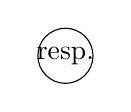
\begin{tikzpicture}[baseline=(t.base)]\node (t) {\unsure{resp.}};\draw (0,0) circle (.35);\end{tikzpicture}}}\\
nG&=G\quad\text{puisque}\quad\deleted{\unsure{par}}\ nB=B,\ nT=T\quad(\text{ce dernier résulte de }{}_n\unsure{M|M'}=0
\end{aligned}\right.
\]

\margin{donne aussi autre \unsure{interprét\textsuperscript{tion}} de ${}_nA$, via hom. cobord si $nG=G$}
\figure{\begin{tikzpicture}\draw (0,0)--(0,1.7);\end{tikzpicture}}
\diagram{\begin{tikzcd}[ampersand replacement=\&, column sep=small]
0 \arrow[r] \& \underset{\underbrace{\vphantom{G}}_{(D(M'_n),{}_nB),\ \text{si }nT=T}}{ {}_nG} \arrow[r] \& {}_nA \arrow[r] \& M_n \arrow[r] \& 0
\end{tikzcd}}

et \unsure{on a de $\widehat{\mathrm m}$} une suite exacte
\diagram{\begin{tikzcd}[ampersand replacement=\&, column sep=small]
0 \arrow[r] \& {}_nG' \arrow[r] \& {}_nA' \arrow[r] \& M'_n \arrow[r] \& 0
\end{tikzcd}}

sous les hyp. duales; passant à la limite sur $n=\ell^\nu$, on a
\[
\left\{\begin{gathered}
\diagram{\begin{tikzcd}[ampersand replacement=\&, column sep=small]0 \arrow[r] \& T_\ell(\unsure{G}) \arrow[r,no head] \& T_\ell(A) \arrow[r] \& M\otimes\unsure{\mathbb Z|\mathbf Z}_\ell \arrow[r,no head] \& 0\end{tikzcd}}\\
\diagram{\begin{tikzcd}[ampersand replacement=\&, column sep=small]0 \arrow[r,no head] \& T_\ell(\unsure{A'|G'}) \arrow[r,no head] \& T_\ell(A') \arrow[r,no head] \& M'\otimes\unsure{\mathbb Z|\mathbf Z}_\ell \arrow[r] \& 0\end{tikzcd}}
\end{gathered}\right.
\]
\margin{30}
